\section{Historical: Focused Compact-Controller Comparison}
\label{sec:suppcompact}
This follow-up tests whether the 188-parameter controller adds value over
smaller learned controls. All four arms use spectral initialization and ten
relaxed Rician EM stages. The step-only arm learns ten update parameters.
The 30-parameter arm adds two filtering parameters per stage. The original
188-parameter arm uses its shared 8--16--2 controller. The new recurrent
arm uses the same smooth Hankel filter but a different controller. We
reuse the original selected checkpoints for the first three arms and
train only the recurrent arm. This is a comparison of fixed designs, not
a search for the best compact network.

\subsection{Residual-Driven Recurrent Control}
Let $G^{t-1}$ be the current estimate, $G_{\rm EM}^t$ its exact EM update,
and
\begin{equation}
 G_{\rm dc}^t=G^{t-1}+\gamma_t(G_{\rm EM}^t-G^{t-1}),\qquad
 \gamma_t=2\operatorname{sigmoid}(a_t).
\end{equation}
The first controller input is shared by users within the received block;
the second is specific to user $k$:
\begin{align}
 r_t&=\log\!\left(1+
 \frac{\|Z-|G_{\rm dc}^tS+B|\|_F^2}{NPv}\right),\\
 u_{tk}&=\log\!\left(1+
 \frac{\|g_{{\rm EM},k}^t-g_k^{t-1}\|_2^2/N}
 {\max\{\|g_{{\rm dc},k}^t\|_2^2/N,10^{-12}\}}\right).
\end{align}
Both inputs use only observations and the current estimate. A shared LSTM
cell takes $(r_t,u_{tk})$ and has four hidden coordinates. Its hidden and
memory states start at zero for every block and every user. States pass
between stages, never between blocks or users. A linear map of the hidden
state gives two outputs $(o_{tk,1},o_{tk,2})$, with
\begin{equation}
 \tau_{{\rm rel},tk}=0.001+\operatorname{softplus}(o_{tk,1}),\qquad
 \beta_{tk}=\operatorname{sigmoid}(o_{tk,2}).
\end{equation}
The smooth singular-value rule is $s\mapsto s^3/(s^2+\tau^2)$, with
$\tau=\tau_{{\rm rel},tk}\|\mathcal H(g_{{\rm dc},k}^t)\|_F/\sqrt q$.
Antidiagonal averaging gives $g_{{\rm str},k}^t$, and the next estimate is
$g_k^t=g_{{\rm dc},k}^t+\beta_{tk}(g_{{\rm str},k}^t-g_{{\rm dc},k}^t)$.
The LSTM has 128 parameters, its output map has ten, and the ten EM steps
give 148 in total. Initial relative strength and mixing are both 0.1;
initial $\gamma_t$ is one.

NA-ALISTA uses observable residual and backprojected-residual summaries
to control linear sparse recovery~\cite{behrens2021naalista}. Our adaptation
instead controls a Hankel filter inside Rician EM. It uses the normalized
inputs above, zero initial recurrent states, hidden-state readout, and
softplus/sigmoid outputs. It learns filtering strength and mixing, not
NA-ALISTA's target-dependent update step. The ten EM steps remain learned
stage constants. Its loss uses withheld magnitudes rather than true
signals. Results therefore concern this adaptation, not reproduction or
superiority over published NA-ALISTA. Input features and architecture both
differ from the 188-parameter arm, so this test alone does not isolate
which difference causes a gain.

\subsection{Matched Training and Fresh Testing}
Each learned arm uses 16,384 observation-only training blocks, 2,048
separate validation blocks, 20 epochs, Adam with learning rate 0.001,
batch size 32, and seeds 9101--9103. Training uses single precision.
For zero-based epoch $e$ and training seed $s$, the mask seed is
$s+10000+e$ and the batch-permutation seed is $s+20000+e$. These match
the original arms. Each mask gives 21 fitting and nine withheld pilots.
Validation masks use seed 2026092203. Checkpoint selection includes epoch
zero and minimizes the equal-weight mean held-out Rician loss over the
126 validation strata. Stratum labels balance offline selection; they
are not controller inputs. No true channels select checkpoints. All
three seeds are retained. They share one training dataset, not three
independent training populations.

Source and development-data hashes are frozen before training. Selected
checkpoint hashes are frozen before new test observations are generated.
Test-bank master seeds are 20261012110001 and 20261012120001. In each bank,
cell $c$ uses world indices $16c$ through $16c+15$. Trial IDs retain both
master seed and index. The 126 primary cells cross SNR $-10$ to 20~dB in
5~dB steps, RSR $5,12,20$~dB, and six path regimes: independently drawn
3--7 paths per user, or fixed $2,4,8,12,16$ paths. Here $N=32$, $K=3$ and
$P=30$. Two extra cells test RSR 0~dB at SNR 5~dB and SNR 60~dB at RSR
12~dB; they are excluded from the primary average. Both use random 3--7
paths. The total is 4,096 fresh paired blocks. Every method receives the
same channel, pilots, reference and noise realization. Inference uses
all 30 pilots, retaining the original change from 21 fitting pilots
during training. This follow-up does not resolve that change separately.

Offline-tuned OptShrink and per-block in-loop rank selection provide
classical context. Their earlier validation-selected settings remain
frozen; no new classical tuning uses these tests.

\subsection{Reporting, Cost and Verification}
For each cell and trained model, we calculate dB NMSE from summed squared
channel error divided by summed true-channel energy across both banks.
The primary statistic averages equally over 126 cells and then over
three training seeds. The three predefined contrasts compare the
188-parameter arm with the step-only, 30-parameter and recurrent arms.
We use 4,000 paired bootstrap resamples within each bank and cell,
retaining pairing across all methods and seeds. Two-sided percentile
intervals use tail probability $0.05/(2\cdot3)$ for a nominal 95\%
Bonferroni familywise level. They are conditional on the fitted models
and development data; they do not measure uncertainty from new training
datasets. Classical comparisons are descriptive in this follow-up.
We also report per-cell results, seed and bank variation, worst-cell
deterioration, pooled NMSE, and fractions with NMSE above $0.5,1,2$.

Timing uses single-thread PyTorch CPU, double precision and batch size
one after training has ended. One independent block per cell uses seed
20261012130001. After warmup, each method runs three times in randomized
order. Times include initialization, controller features, filtering,
rank search and refitting, but exclude model loading and file access
for every method. Training cost is separate. These are measured
implementation times, not hardware-independent complexity claims.

Verification checks parameter counts, constant-control equivalence,
finite outputs and gradients, a central-difference gradient, single/double
precision agreement, state reset, user permutation, and deterministic
optimizer resumption. The result audit regenerates all test inputs,
checks hashes and trial IDs, replays one prediction per model and
cell/bank, compares classical predictions with an independent NumPy
implementation every eighth cell, and recalculates headline statistics
with scalar sums. No outcome is inferred from these checks before the
complete result audit.

\subsection{Full Compact-Control Results}

\begin{table}[!t]
\caption{Fresh matched compact comparison: 4,032 primary worlds and 64 separate stress worlds. Lower NMSE is better. Neural scores average three models, not an ensemble. All timings include initialization, use one PyTorch CPU thread and count rank search/refitting.}
\label{tab:compact}\centering\footnotesize
\setlength{\tabcolsep}{3pt}
\begin{tabular}{@{}lrrr@{}}\toprule
Method & Weights & NMSE (dB) & Time (ms)\\
\midrule
Learned steps only & 10 & -9.773 & 1.79\\
Global filtering & 30 & -11.857 & 3.41\\
Spectral/state controller & 188 & -13.692 & 4.87\\
Recurrent control & 148 & -11.725 & 4.15\\
OptShrink, offline & --- & -13.204 & 15.81\\
OptShrink, block rank & --- & -14.144 & 110.56\\
\bottomrule
\end{tabular}
\end{table}


\begin{table}[!t]
\caption{188-parameter gains: positive favors the spectral/state controller. Three predeclared comparisons with Bonferroni-adjusted paired intervals. Worst-cell harm is descriptive, not an upper confidence bound.}
\label{tab:compact-contrasts}\centering\footnotesize
\setlength{\tabcolsep}{3pt}
\begin{tabular}{@{}lrrr@{}}\toprule
Comparator & Gain (dB) & 95\% interval & Worst harm\\
\midrule
Learned steps only & +3.919 & [+3.789, +4.001] & 2.735\\
Global filtering & +1.835 & [+1.805, +1.871] & 0.580\\
Recurrent control & +1.967 & [+1.932, +2.006] & 0.176\\
\bottomrule
\end{tabular}
\end{table}


\begin{table}[!t]
\caption{Different error summaries on the same primary worlds. Pooled NMSE pools linear errors before taking dB and is not the primary score. Threshold rates are percentages.}
\label{tab:compact-tails}\centering\footnotesize
\setlength{\tabcolsep}{3pt}
\begin{tabular}{@{}lrrrr@{}}\toprule
Method & Pooled (dB) & $>.5$ & $>1$ & $>2$\\
\midrule
Learned steps only & -1.651 & 29.99 & 22.84 & 14.24\\
Global filtering & -2.438 & 27.98 & 19.56 & 12.52\\
Spectral/state controller & -6.664 & 19.43 & 3.10 & 0.00\\
Recurrent control & -2.396 & 28.04 & 19.78 & 12.62\\
OptShrink, offline & -6.564 & 19.12 & 4.46 & 0.00\\
OptShrink, block rank & -6.228 & 19.27 & 6.77 & 0.27\\
\bottomrule
\end{tabular}
\end{table}


\begin{table}[!t]
\caption{Separate stress tests, 32 paired worlds each. Weak reference: SNR 5/RSR 0 dB. Nearly noiseless: SNR 60/RSR 12 dB. Neither enters selection or the primary average.}
\label{tab:compact-stress}\centering\footnotesize
\setlength{\tabcolsep}{3pt}
\begin{tabular}{@{}lrr@{}}\toprule
Method & Weak reference & Nearly noiseless\\
\midrule
Learned steps only & -4.065 & -44.417\\
Global filtering & -6.505 & -30.975\\
Spectral/state controller & -6.842 & -6.321\\
Recurrent control & -5.623 & -20.101\\
OptShrink, offline & -10.823 & -67.701\\
OptShrink, block rank & -12.625 & -70.336\\
\bottomrule
\end{tabular}
\end{table}


\begin{table}[!t]
\caption{Primary scores by training initialization. These seeds share the same training data and do not represent independent training populations.}
\label{tab:compact-seeds}\centering\footnotesize
\setlength{\tabcolsep}{3pt}
\begin{tabular}{@{}lrrr@{}}\toprule
Method & 9101 & 9102 & 9103\\
\midrule
Learned steps only & -9.770 & -9.774 & -9.774\\
Global filtering & -11.852 & -11.853 & -11.865\\
Spectral/state controller & -13.784 & -13.449 & -13.843\\
Recurrent control & -11.707 & -11.740 & -11.728\\
\bottomrule
\end{tabular}
\end{table}


\begin{table}[!t]
\caption{Recurrent training records. Time includes validation and parallel-worker contention; it is not an isolated-device training benchmark.}
\label{tab:compact-training}\centering\footnotesize
\setlength{\tabcolsep}{3pt}
\begin{tabular}{@{}rrrr@{}}\toprule
Seed & Selected epoch & Held-out NLL & Minutes\\
\midrule
9101 & 20 & 3.43585 & 17.37\\
9102 & 19 & 3.43353 & 17.09\\
9103 & 20 & 3.43426 & 17.34\\
\bottomrule
\end{tabular}
\end{table}


The audit regenerated all 4,096 test worlds, replayed 3,072 representative neural predictions and independently replayed 64 classical predictions in NumPy. Maximum absolute replay difference was $4.40e-13$. Headline scores were also recomputed with scalar loops. These numerical checks do not establish statistical optimality or global recovery.

\begin{figure*}[!t]\centering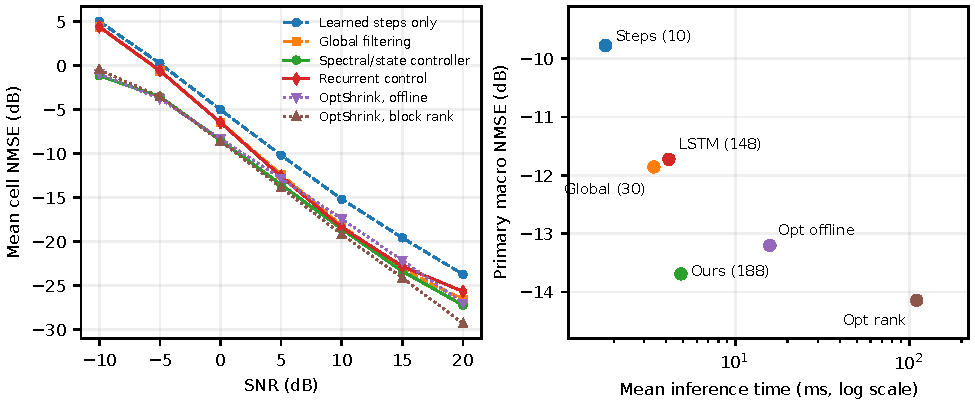
\includegraphics[width=\textwidth]{compact_comparison.pdf}\caption{Fresh compact-control comparison. Left: each SNR point averages 18 reference/path cells. Right: primary accuracy and measured serial inference time. These descriptive summaries do not imply cellwise confidence guarantees.}\label{fig:compact}\end{figure*}

